\chapter{Evaluation}
\label{ch:evaluation}

This chapter contains the evaluation of the methods proposed in the previous part, chapter~\ref{ch:reducing}. In section~\ref{sec:setup}, we present the data sets and the methodology used for testing. We give details about the parameter choices and set baseline scores obtained by either classical NCA or simple linear projections, such as PCA, LDA or RCA. Results for each individual method are presented in sections~\ref{sec:method-comparison} and~\ref{sec:eval-nca-approx}. A comparison of the methods is shown in subsection~\ref{subsec:eval-comparison} using accuracy versus time plots.

We should mention that we did not include all the results in this chapter to prevent cluttering. Further experimentations can be found in appendix~\ref{app:results}.

\section{Evaluation setup}
\label{sec:setup}

The evaluation was done in terms of two metrics: accuracy and speed. An additional and more subjective criterion is to judge a method by visualizing low dimensional representations of various data sets. We provided 2D plots of the projected data where suitable.

The data sets selected for testing are listed in table~\ref{tab:datasets}. We note that the used data vary both in number of samples~$N$ and in dimensionality~$D$. Even if we concentrate on large amounts of data, we need small data sets to assess the performance of the new models. The methods' speed was tested on the large data sets (\texttt{usps}, \texttt{magic} and \texttt{mnist}). However, the diversity in size and complexity made it difficult to find the optimal selection of parameters. We are aware that there is ``no free lunch'' in accurately solving widely different problems with a fixed model. When concentrating on a single task it is often advised to include prior knowledge into the model. 
% Also it is easier to make minor tweaks of the parameters to boost the performance.

\begin{table}%`
  \centering
    \begin{tabular}{l l c c c} \toprule
	Data set name&Abbrevation&$N$&$D$&$C$\\ 
	\midrule
	Balance scale&\texttt{balance}&$625$&$4$&$3$\\ 
	Ecoli&\texttt{ecoli}&$336$&$7$&$8$\\ 
% 	&\texttt{fruit}&$59$&$3$&$3$\\ 
	Glass identification&\texttt{glass}&$214$&$9$&$6$\\ 
	Ionosphere&\texttt{ionosphere}&$351$&$33$&$2$\\ 
	Iris&\texttt{iris}&$150$&$4$&$3$\\ 
	Landsat satellite&\texttt{landsat}&$6435$&$36$&$6$\\ 
	MAGIC Gamma telescope&\texttt{magic}&$19020$&$10$&$2$\\ 
	MNIST digits&\texttt{mnist}&$70000$&$784$&$10$\\ 
% 	&\texttt{olivetti}&$400$&$4096$&$40$\\ 
	Pima Indians diabetes&\texttt{pima}&$768$&$8$&$2$\\ 
	Image segmentation&\texttt{segment}&$2310$&$18$&$7$\\ 
%	SPECTF heart&\texttt{spectf}&$267$&$44$&$2$\\ 
	Blood transfusion&\texttt{transfusion}&$748$&$4$&$2$\\ 
	USPS digits&\texttt{usps}&$11000$&$256$&$10$\\ 
	Wine&\texttt{wine}&$178$&$13$&$3$\\ 
	Yeast&\texttt{yeast}&$1484$&$8$&$10$\\  
      \bottomrule
    \end{tabular}
    \caption[List of the data sets used for evaluation]{This table presents the characteristics of the data sets used: number of samples $N$, dimensionality of the data $D$ and number of classes $C$. The two digits data sets \texttt{mnist} and \texttt{usps} were downloaded from the following URL \protect\url{http://cs.nyu.edu/~roweis/data.html}. All the others data sets are available in the UCI repository \protect\url{http://archive.ics.uci.edu/ml/datasets.html}.}
    \label{tab:datasets}
\end{table}

For evaluation we used $70\%$ of each data set for training and the remaining $30\%$ was kept for testing. We report standard errors for the mean accuracy averaged over different splits.
We made exceptions for two data sets: \texttt{landsat} and \texttt{mnist}. These are already split into standard training and testing sets. 

The methods we test are: sub-sampling (SS; section~\ref{sec:sub-sampling}), mini-batches (MB; section~\ref{sec:mini-batches}), stochastic learning (SL; section~\ref{sec:stochastic-learning}). For stochastic learning we included two approximated method: the fast kernel density estimation idea (SL-KDE; section~\ref{sec:approximate}) and compact support version of NCA (SL-CS; section~\ref{sec:exact-computations}). Each method has particular parameters that we discuss in its corresponding subsection. 

There are some common choices for all the methods, related to the NCA implementation. For convenience, we review these choices here. We experimented with three optimization methods: gradient ascent with the ``bold driver'' heuristic, conjugate gradients and variants of stochastic gradient ascent with ``early stopping''. For initialization we used the techniques described in subsection~\ref{subsec:initialization}: random initialization, principal component analysis (PCA; \citealp{pearson1901}), linear discriminant analysis (LDA; \citealp{fisher1936}) or relevant component analysis (RCA; \cite{bar2003}). At test time, we did classification using $1$-NN or using an NCA based function as described in subsection~\ref{subsec:doing-classification}. However, we usually present scores using both classification rules.

The experiments were carried in \textsc{Matlab} and most of the implementations are the authors' own work. There are some exceptions however. For conjugate gradients (CG) we used the function \texttt{minimize.m}, written by \citet{rasmussen-online}.\footnote{This is available for download at $<$\url{http://www.gaussianprocess.org/gpml/code/matlab/util/minimize.m}$>$.}
 The RCA implementation was provided by Noam Shental on his web-page.\footnote{The code was downloaded from $<$\url{http://www.openu.ac.il/home/shental/}$>$.}
 Also we used functions from Iain Murray's \textsc{Matlab} toolbox.\footnote{Iain Murray's toolbox is available at $<$\url{http://homepages.inf.ed.ac.uk/imurray2/code/imurray-matlab/}$>$.} Finally, we inspected previous implementations of NCA,\footnote{Implementations of NCA are provided by Laurens van der Maaten in his \textsc{Matlab} Toolbox for Dimensionality Reduction $<$\url{http://homepage.tudelft.nl/19j49/Matlab_Toolbox_for_Dimensionality_Reduction.html}$>$ and by Charless C. Fowlkes on his website $<$\url{http://www.ics.uci.edu/~fowlkes/software/nca/}$>$.}
 even if we did not explicitly make use of them.

\section{Baseline}
\label{sec:baseline} 

We started by implementing the standard NCA algorithm (appendix \ref{app:code-nca-obj}). This is the main baseline against which we compare new models.  
For our first series of experiments, we tried to replicate the work in the original article \citep{goldberger2004}. We encountered some difficulties since no information about their implementation was provided in the paper. Our results are presented in table \ref{table:eval-baseline} (scores are averaged over 40 runs). We randomly initialized the matrix~$\AB$ and optimized it using conjugate gradients (CG) method. This was the easiest thing to do since no parameter tuning is need for CG. We note that the results are similar to those of \citet{goldberger2004}; for the \texttt{ionosphere} data set we obtained slightly worse results.

\begin{table}
  \centering\begin{tabular}{lrcccc}
  \toprule
	  &     & Train score  & \multicolumn{2}{c}{Test scores} & Baseline \\
  \cmidrule(r){3-3} \cmidrule(r){4-5} \cmidrule(r){6-6}
  Data set & $d$ & $f(\AB)$ & $1$-NN & NCA & Eucl. \\
  \midrule
    \texttt{balance}&$2$&$92.86 \pm 0.47$&$90.78 \pm 0.53$&$90.61 \pm 0.55$&\\ 
		    &$D=4$&$95.36 \pm 0.38$&$93.40 \pm 0.47$&$93.04 \pm 0.51$&$76.18$\\ 
    \midrule
    \texttt{ionosphere}&$2$&$98.31 \pm 0.14$&$79.86 \pm 0.75$&$79.74 \pm 0.78$&\\ 
		       &$D=33$&$72.07 \pm 0.71$&$86.22 \pm 0.64$&$72.87 \pm 0.71$&$85.38$\\ 
    \midrule
    \texttt{iris}&$2$&$99.38 \pm 0.11$&$94.94 \pm 0.39$&$94.72 \pm 0.39$&\\ 
		 &$D=4$&$99.48 \pm 0.10$&$95.10 \pm 0.44$&$95.15 \pm 0.44$&$95.53$\\
    \midrule
    \texttt{wine}&$2$&$99.15 \pm 0.14$&$92.4 \pm 1.0$&$92.4 \pm 1.0$&\\ 
		 &$D=13$&$98.95 \pm 0.15$&$95.36 \pm 0.51$&$95.36 \pm 0.51$&$74.53$\\ 
  \bottomrule
  \end{tabular}
  \caption[NCA accuracy on four small data sets]{Accuracy of standard NCA on four small data sets. Scores are averaged over 40 runs. The second column presents the dimensionality~$d$ the data set is reduced to. The last column shows the leave one out cross validation performance on the data set using Euclidean metric.}
  \label{table:eval-baseline}
\end{table}

\begin{table}
  \centering\begin{tabular}{lccc}
  \toprule
  Data set & PCA & LDA & RCA \\
  \cmidrule(r){2-4}
\texttt{usps}&$73.47 \pm 0.13$&$87.44 \pm 0.12$&$87.42 \pm 0.13$\\ 
\texttt{magic}&$77.097 \pm 0.080$&$76.17 \pm 0.29$&$77.574 \pm 0.078$\\ 
\texttt{mnist}&$70.13$&$9.96$&$79.11$\\
\bottomrule
  \end{tabular}
  \caption[Accuracy of PCA, LDA and RCA on large data sets]{Accuracy of three linear transformation techniques applied on the large data sets. We used $1$-NN for classification. Scores are averaged over 20 runs, except for \texttt{mnist} data set. We reduced each data set dimensionality to $d=5$.}
  \label{table:eval-baseline-large-data-sets}
\end{table}
% We used as a baseline a standard NCA implementation . 
% This allowed us to have a baseline to compare the new models against, table \ref{table:eval-baseline}.
% We started testing NCA on small data sets.  This can also be viewed as a replication of the work in the original article \citet{goldberger2004}. The authors did not provide us with any information about their implementation. For our first series of experiments, we used random initialization and we optimized the function using conjugate gradients. The results are averaged over 40 runs. We also considered the score obtained in the original space. We computed this using leave one out cross validation using the Euclidean metric. The results are quite similar to those presented in the original paper.  
% 
% Also for comparison we also offer scores from applying PCA, LDA and RCA followed by $1$-NN.

However, in order to achieve a robust implementation of NCA we had to carry out additional experiments. The lessons learnt were summarized in section~\ref{sec:practical-notes}. We will further see the influence of the implementation tricks in the next part (section~\ref{sec:method-comparison}). Results were shown in section~\ref{sec:practical-notes} and are also attached at the end of the thesis, appendix~\ref{app:results}:
\begin{itemize}
 \item Tables~\ref{table:comp-opts-1} and~\ref{table:comp-opts-2} compare two of the optimization methods: conjugate gradients and gradient ascent with the ``bold driver'' heuristic. We observe that the two methods give close scores on most of data sets. However, the gradient ascent takes longer until it reaches convergence.
 \item Figures~\ref{fig:iris-init}, \ref{fig:balance-init} and~\ref{fig:ecoli-init} illustrate the initialization effect on three data sets: \texttt{iris}, \texttt{balance} and \texttt{ecoli}. RCA seems to be the best option for initialization and we used it in most of our comparisons. However, random projection can also be sometimes surprisingly good as we see in figure~\ref{fig:iris-init-2}. 
\end{itemize}

We could not apply NCA on large data sets (\texttt{usps}, \texttt{magic}, and \texttt{mnist}) since it would have taken far too long. We decided to use as a baseline the linear transformations that we also use for initialization (PCA, LDA and RCA). The results are averaged over different splits of training and testing set and they are listed in table \ref{table:eval-baseline-large-data-sets}. For the \texttt{mnist} data set we have scores of classic NCA \citep{singh2010}. For $d=5$ the accuracy obtained was $91.1\%$ using the $k$NN classifier and $90.9\%$ using the NCA classifier. For the classification procedure \citeauthor{singh2010} learnt the optimal value for $k$ using cross-validation.

\section{Mini-batches methods}
\label{sec:method-comparison}

 The mini-batch methods were compared on the larger data sets: \texttt{usps}, \texttt{magic}, and \texttt{mnist}. We chose to reduce the dimensionality to $d=5$. This decision was partly motivated by the fact that NCA is very effective for reducing the data dimensionality to small values, somewhere around $5$ to $15$. A more principled approach would have been to develop a model choosing algorithm: start with a projection to $d=2$ dimensions and then increase the number of dimensions until the score stops improving. This idea is similar to the ``early stopping'' procedure, and is illustrated for the \texttt{landsat} data set in figure \ref{fig:landsat-evolution}.

  \begin{figure}
   \centering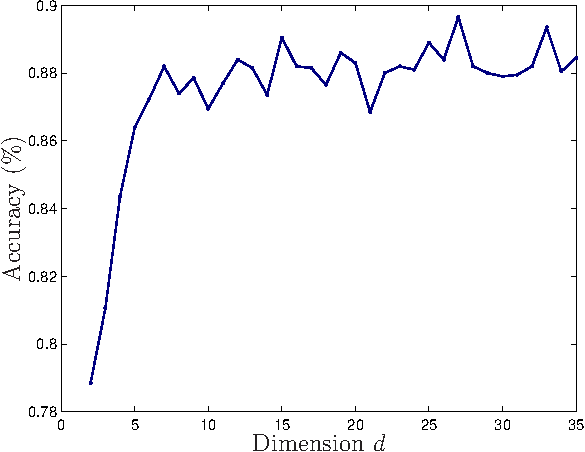
\includegraphics[width=0.6\textwidth]{images/landsat-evolution}
   \caption[Test accuracy as function of reduced dimensionality $d$ on the \texttt{landsat} data]{Evolution of test accuracy as dimensionality increases on \texttt{landsat} data set. We see that NCA operates almost as well in low dimensions ($d=6,\cdots,10$) as in high dimensions ($d>25$). This approach can be used for selecting a suitable dimension to which we project the data.}
   \label{fig:landsat-evolution}
  \end{figure}


  \subsection{Sub-sampling}
  \label{subsec:eval-sub-sampling}

    For sub-sampling we trained NCA on a subset of $n=3000$ samples of the original data. We used conjugate gradients for optimization and RCA linear transformation for initialization. As previously mentioned in section \ref{sec:sub-sampling}, the sub-sampled data has a thinner distribution than the original data which helps the method to obtain good scores at training. But the test performance is hindered because we do not use the true distribution. This is especially evident for the digits data \texttt{usps} and \texttt{mnist} (table \ref{tab:ss}). 
    \begin{table}
    	\centering
    	\begin{tabular}{lccc}
    	\toprule
    	Data set & Train & $1$-NN & NCA \\
    	\cmidrule(r){2-2}\cmidrule(r){3-4}
    	 \texttt{usps}&$99.112 \pm 0.099$&$89.30 \pm 0.18$&$89.41 \pm 0.16$\\
    	 \texttt{magic}&$82.71 \pm 0.41$&$79.25 \pm 0.45$&$80.22 \pm 0.72$\\
    	 \texttt{mnist}&$96.867$&$82.130$&$82.470$\\
    	 \bottomrule
    	\end{tabular}
	\caption[Accuracy for the sub-sampling method on large data sets]{Accuracy scores for the sub-sampling method on the larger data sets. We used RCA for initialization and CGs for optimization. We used a subset of $n=3000$ data points for training and the whole data set for testing.}
	\label{tab:ss}
    \end{table}

    \subsection{Mini-batches}
    \label{subsec:eval-mini-batches}

    We trained NCA using the gradient ascent variant with clustered mini-batches (section~\ref{sec:mini-batches}). For the learning rate, we used an update rule of the form $\frac{\eta}{t+t_0}$. We fixed $\eta=1$ and tuned the other free parameter $t_0$ using cross validation across an exponential scale from $0.1$ to $1000$. After that, a finer tuning was done on a linear scale around the best value of $t_0$. We used $5\%$ of the training set for cross validation to monitor the accuracy score at each iteration. If the performance on the cross validation set does not increase for $25$ iterations, we stop the learning process and return to the previously best parameter.

    To get significant gradients we used large mini-batches $n=2000$. The points in a batch are selected via the recursive projection clustering (RPC; \citealp{chalupka2011}) algorithm. The clustering was done in the low dimensional space, after projecting the points with the current linear transformation matrix~$\AB$.
    The results obtained by the mini-batch method can be found in table \ref{tab:mb}. We note similar scores on \texttt{magic} and better results on the other two data sets.

    \begin{table}
        	\centering
        	\begin{tabular}{lccc}
        	\toprule
        	Data set & Train & $1$-NN & NCA \\
        	\cmidrule(r){2-2}\cmidrule(r){3-4}
        	 \texttt{usps}&$92.00 \pm 0.43$&$91.26 \pm 0.17$&$92.37 \pm 0.17$\\
        	 \texttt{magic}&$80.04 \pm 0.48$&$79.14 \pm 0.52$&$79.8 \pm 1.1$\\
        	 \texttt{mnist}&$87.47 \pm 0.49$&$87.52 \pm 0.36$&$89.88 \pm 0.25$\\
        	 \bottomrule
        	\end{tabular}
		\caption[Accuracy for the mini-batch method on large data sets]{Accuracy scores for mini-batch method on the larger data sets. We used RCA for initialization and the mini-batches were clustered in the low-dimensional space using RPC. The size of a mini-batch was of maximum $n=2000$ data points.}
		\label{tab:mb}
    \end{table}

    \subsection{Stochastic learning}
    \label{subsec:eval-stochastic-learning}

    This method was trained using the variant of stochastic gradient ascent presented in section \ref{sec:stochastic-learning}. We used the same parameters as in the previous section. We considered $n=50$ neighbours to look at for each iteration and computed their contributions with respect to the whole data set. 

    Besides the results on the large data sets (table~\ref{tab:sl-2}), we also present the performance of this method when used for small data sets (table~\ref{tab:sl-1}). We note a considerable improvement on the \texttt{magic} data set compared to the previous two methods. For small data sets, we observe similar results as the baseline NCA. The most important remark is that the classification done using NCA objective function is better than $1$-NN classification. This observation also applies for the large data sets results. More results for this method are in the appendix, table~\ref{app:table:nca-sl-small-1} and~\ref{app:table:nca-sl-small-2}.

    \begin{table}
      \centering\begin{tabular}{lrccc}
      \toprule
	      &     & Train score  & \multicolumn{2}{c}{Test scores}\\
      \cmidrule(r){3-3} \cmidrule(r){4-5}
      Data set & $d$ & $f(A)$ & $1$-NN & NCA \\
      \midrule
	\texttt{balance}&$2$&$88.35 \pm 0.83$&$87.37 \pm 0.49$&$90.45 \pm 0.38$\\  
	&$D=4$&$94.70 \pm 0.87$&$95.32 \pm 0.34$&$96.14 \pm 0.29$\\ 
	\midrule
	\texttt{ionosphere}&$2$&$89.0 \pm 1.7$&$85.71 \pm 0.94$&$87.08 \pm 0.95$\\
	&$D=33$&$92.6 \pm 1.5$&$84.72 \pm 0.57$&$84.34 \pm 0.59$\\ 
	\midrule
	\texttt{iris}&$2$&$96.41 \pm 0.94$&$96.33 \pm 0.57$&$97.00 \pm 0.46$\\ 
	&$D=4$&$97.5 \pm 1.3$&$95.67 \pm 0.71$&$96.11 \pm 0.66$\\ 
	\midrule
	\texttt{wine}&$2$&$98.80 \pm 0.70$&$97.22 \pm 0.65$&$97.50 \pm 0.49$\\ 
	&$D=13$&$99.25 \pm 0.62$&$96.85 \pm 0.41$&$96.85 \pm 0.41$\\ 
      \bottomrule
      \end{tabular}
      \caption[Accuracy for the stochastic learning method on small data sets]{Accuracy scores for stochastic learning method on the small data sets. We used RCA for initialization. The scores are averaged after 20 iterations.}
    \label{tab:sl-1}
    \end{table}

        \begin{table}
            	\centering
            	\begin{tabular}{lccc}
            	\toprule
            	Data set & Train & $1$-NN & NCA \\
            	\cmidrule(r){2-2}\cmidrule(r){3-4}
            	\texttt{usps}&$90.23  \pm 0.50$&$90.68 \pm 0.22$&$92.64 \pm 0.17$\\
            	\texttt{magic}&$78.39 \pm 0.25$&$79.76 \pm 0.13$&$84.49 \pm 0.12$\\
            	\texttt{mnist}&$85.97 \pm 0.37$&$86.07 \pm 0.43$&$89.35 \pm 0.39$\\
            	 \bottomrule
            	\end{tabular}
		\caption[Accuracy for the  stochastic learning method on large data sets]{Accuracy scores for stochastic learning method on the larger data sets. We used RCA for initialization. At each iteration we considered $n=50$ data points.}
		\label{tab:sl-2}
        \end{table}

    \subsection{Comparison}
    \label{subsec:eval-comparison}

    To easily compare the three methods presented, we provide time-accuracy plots (figure \ref{fig:time-accuracy}). We did not record the time taken for smaller data sets, since the classical NCA was usually fast enough. We also included in the plots the method based on the compact support kernels (we discuss its individual scores in subsection \ref{subsec:eval-nca-cs}). 

    In terms of accuracy, all of the NCA variants improve the accuracy over PCA, LDA or RCA\@. Sub-sampling gives comparable results to the other two methods only on the \texttt{magic} data set. This data set has only two classes and a sub-sampled data set does not remove too much information about the decision boundaries. Mini-batches and stochastic learning are similar in accuracy. The proposed methods obtain a slightly worse score than classic NCA on \texttt{mnist}. The performance reported by \citet{singh2010} was around $91\%$, while the mean accuracy for these two methods is about $90\%$. 

    The differences in time varied strongly. We used a logarithmic scale on the time to better discriminate the plotted scores. For each method we show the equidensity contours of the Gaussian distribution. The contours are ellipses, but because of the logarithmic axis they look deformed. 

    The time spent varies even for the same method because the number of iterations until convergence depends on random parameters. We notice a certain trade-off between time and accuracy, especially for the digits data sets.

    We also show low dimensional representations of the data sets for $d=2$ for \texttt{usps} (figure \ref{fig:usps-projection}) and \texttt{magic} (figure \ref{fig:magic-projection}). 
    
      \begin{figure}
		\centering
		\subfigure[\texttt{usps}]{\label{fig:usps}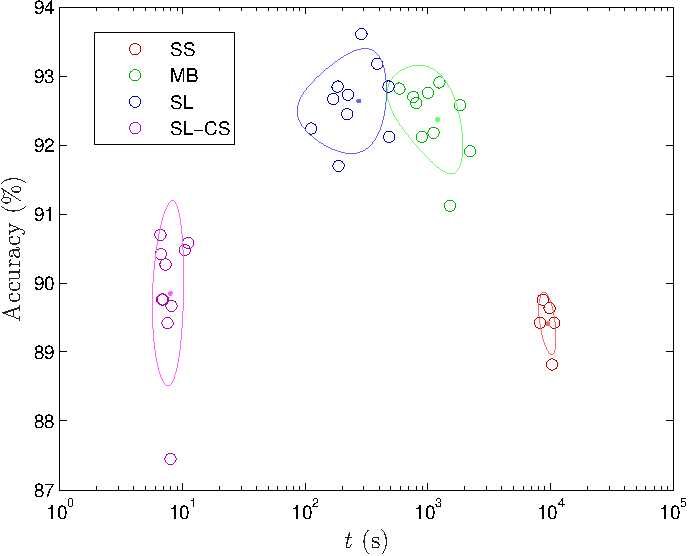
\includegraphics[width=0.55\textwidth]{images/usps-acc-time}}
		\subfigure[\texttt{magic}]{\label{fig:magic}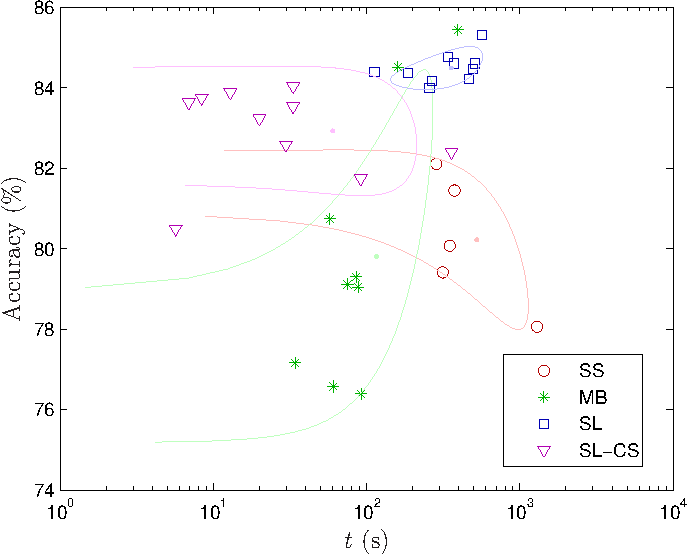
\includegraphics[width=0.55\textwidth]{images/magic-acc-time}}
		\subfigure[\texttt{mnist}]{\label{fig:mnist}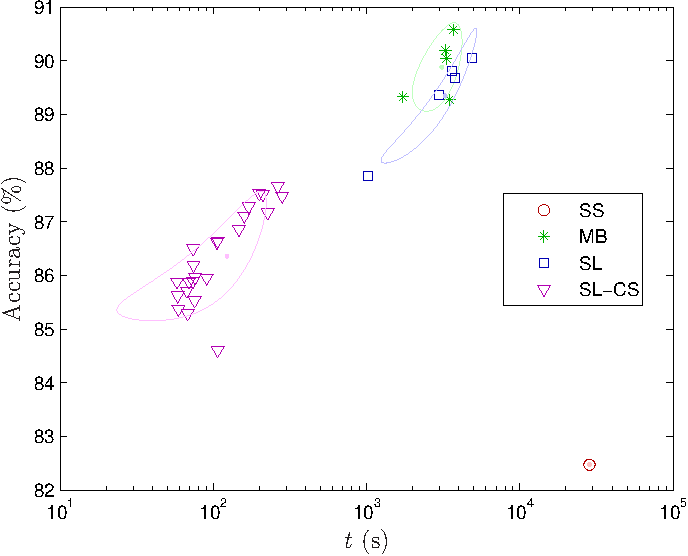
\includegraphics[width=0.55\textwidth]{images/mnist-acc-time}}
		\caption[Time vs. accuracy plots for four of the methods proposed: sub-sampling, mini-batches, stochastic learning and stochastic learning for compact support NCA]{Time vs. accuracy plots on larger data sets for four of the proposed methods: sub-sampling (SS), mini-batches (MB), stochastic learning (SL) and stochastic learning with compact support NCA (SL-CS). For SS we plotted the $1$-NN score, while for the other three the points indicate the NCA score.}
		\label{fig:time-accuracy}
      \end{figure}

     \begin{figure}
		 \centering
			  \subfigure[Mini-batch method]{\label{fig:nca-mb-usps}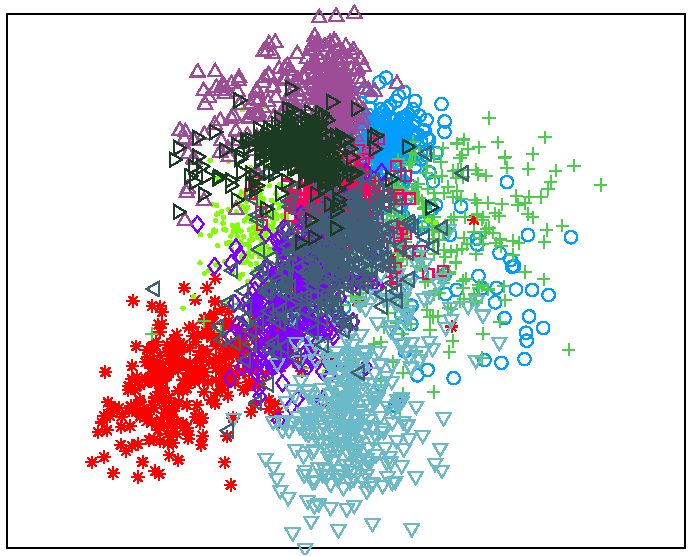
\includegraphics[width=0.45\textwidth]{images/usps-test-mb}}
			    \hspace{0.02\textwidth}
			 \subfigure[Stochastic learning]{\label{fig:nca-sl-usps}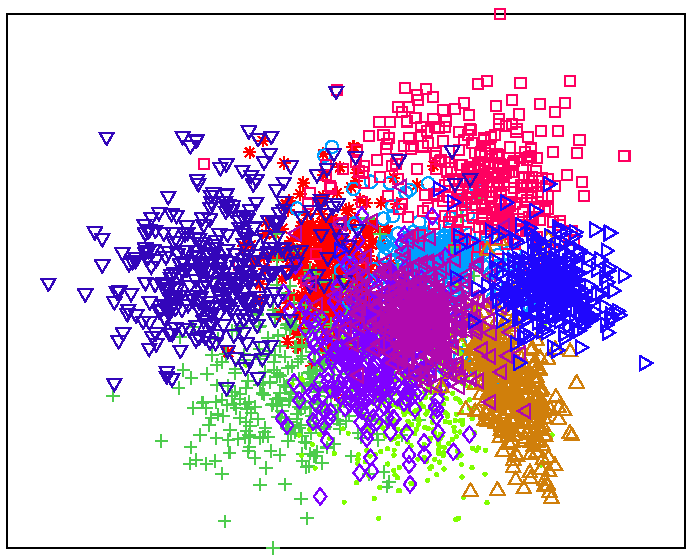
\includegraphics[width=0.45\textwidth]{images/usps-test-snca}}
		\caption[Two dimensional projections of \texttt{usps} data set using two variants of NCA learning: mini-batches and stochastic learning]{Two dimensional projections of \texttt{usps} data set using two variants of NCA learning. The linear transformation was learnt on a training set, and here is plotted the projection of a testing set.}
		\label{fig:usps-projection}
	\end{figure}

     \begin{figure}
		 \centering
			  \subfigure[Mini-batch method]{\label{fig:nca-mb-magic}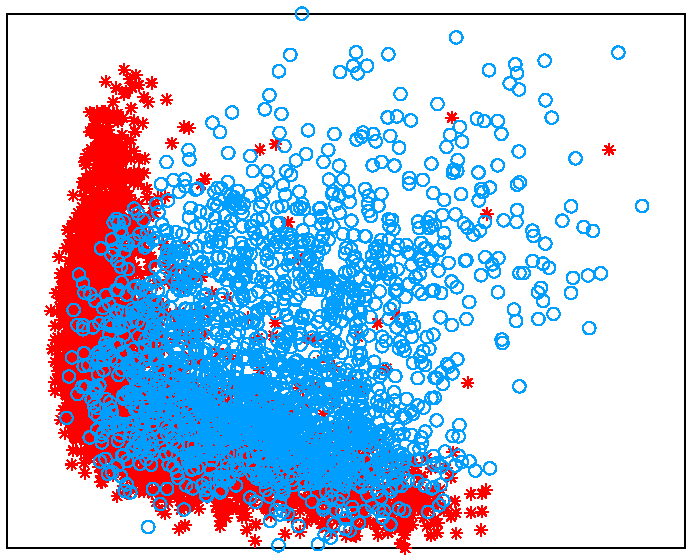
\includegraphics[width=0.45\textwidth]{images/magic-test-mb}}
			    \hspace{0.02\textwidth}
			 \subfigure[Stochastic learning]{\label{fig:nca-sl-magic}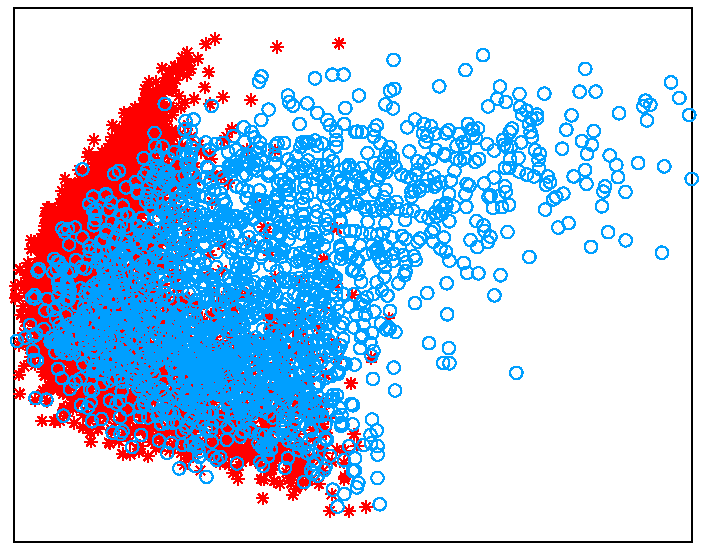
\includegraphics[width=0.45\textwidth]{images/magic-test-snca-cs}}
		\caption[Two dimensional projections of \texttt{magic} data set using two variants of NCA learning: mini-batches and stochastic learning]{Two dimensional projections of \texttt{magic} data set using two variants of NCA learning. The linear transformation was learnt on a training set, and here is plotted the projection of a testing set.}
		\label{fig:magic-projection}
	\end{figure}

\section{Approximate computations}
\label{sec:eval-nca-approx}

The following methods can be applied on classic NCA, but we tested them in conjunction with the stochastic learning procedure to further boost the speed. 

For approximate computations we also tried a more simplistic approach, similar to that of \citet{weinberger2007}: we selected only the first $100$ neighbours for each point and discarded those points whose contribution~$p_{ij}$ is less than $\exp(-30)$. This simple approach gave surprisingly good scores, although we do not present them here.

\subsection{NCA with $k$-d trees}
\label{subsec:eval-nca-k-d-trees}

For the class-conditional kernel density estimation idea we used the algorithm described in section \ref{sec:approximate}. Our $k$-d tree implementation was written in \textsc{Matlab} and, for this reason, it was pretty slow. The code was slower than the simple SL version, because we could not vectorize the recursive computation of the objective function and its gradient. We experimented with kernel density code written in C and mex-ed in \textsc{Matlab} and we think that such an approach can improve the speed. Doing simple kernel density estimation with a C written code proved to be even faster than doing it in \textsc{Matlab}. The short time did not permit us to finalize this approach. We demonstrate that SL with $k$-d trees achieves good results even if we discard a large number of the points. Table \ref{tab:nca-sl-k-d-trees} shows results for this method on the large data sets. We also present how the accuracy and the average number of prunings depend on the maximum error imposed (table \ref{tab:nca-sl-k-d-trees-landsat}). 

\begin{table}
  \centering
 	\begin{tabular}{lcccc}
 	\toprule
 	$\epsilon_{\max}$ & Train & $1$-NN & NCA & Visited points\\
 	\cmidrule(r){2-2}\cmidrule(r){3-4}\cmidrule(r){5-5}
$0$&$87.05 \pm 0.66$&$86.30 \pm 0.32$&$87.87 \pm 0.24$&$80.0 \pm 5.9$\\
$10^{-50}$&$87.50 \pm 0.31$&$86.26 \pm 0.24$&$87.88 \pm 0.20$&$55.1 \pm 5.2$\\
$10^{-20}$&$85.49 \pm 0.89$&$86.32 \pm 0.28$&$87.87 \pm 0.26$&$45.7 \pm 4.1$\\
$10^{-5}$&$87.29 \pm 0.49$&$85.95 \pm 0.19$&$87.63 \pm 0.29$&$22.8 \pm 2.7$\\
$0.01$&$87.34 \pm 0.76$&$86.14 \pm 0.29$&$87.90 \pm 0.24$&$22.1 \pm 4.2$\\
$0.1$&$86.70 \pm 0.39$&$86.12 \pm 0.29$&$88.09 \pm 0.19$&$20.0 \pm 2.0$\\
\bottomrule
  \end{tabular}
  \caption[Accuracy for the  approximated version of NCA trained using stochastic learning on the \texttt{landsat} data set]{Stochastic learning for the approximated version of NCA that uses $k$-d trees. The data set used is \texttt{landsat}. $\epsilon_{\max}$ denotes the maximum error that we accept while approximating the density for a point given a class~$p(\xB|c)$. `Visited points' indicates the fraction of points that are used for computing the function and the gradient.}
  \label{tab:nca-sl-k-d-trees-landsat}
\end{table}


\begin{table}
  \centering
 	\begin{tabular}{lccc}
 	\toprule
 	Data set & Train & $1$-NN & NCA \\
 	\cmidrule(r){2-2}\cmidrule(r){3-4}
 	\texttt{usps}&$89.68 \pm 0.51$&$90.57 \pm 0.20$&$92.67 \pm 0.15$\\
\texttt{magic}&$78.09 \pm 0.37$&$79.68 \pm 0.30$&$84.50 \pm 0.21$\\
\texttt{mnist}&$84.4 \pm 1.4$&$85.5 \pm 1.0$&$88.98 \pm 0.75$\\
  \bottomrule
  \end{tabular}
  \caption[Accuracy for the  approximated version of NCA trained using stochastic learning on large data sets]{Stochastic learning for the approximated version of NCA that uses $k$-d trees. For these experiments we set $\epsilon_{\max}=0.1$.}
  \label{tab:nca-sl-k-d-trees}
\end{table}

\subsection{NCA with compact support kernels}
\label{subsec:eval-nca-cs}

\begin{figure}
	\centering
	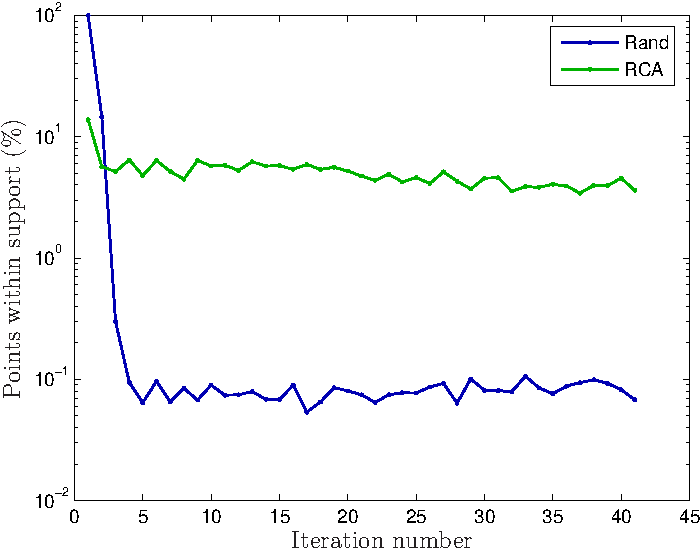
\includegraphics[width=0.6\textwidth]{images/nca-cs-nnzs}
	\caption[Fraction of the points visited during the training of the compact support NCA ]{This figure illustrates how the fraction of the points inspected varies during the learning procedure. When we use random initialization, there are inspected only $0.1\%$ of the points. If RCA is used to initialize the learning algorithm a fraction of about $10\%$ is used.}
	\label{fig:nca-cs-nnzs}
\end{figure}
\begin{figure}
		 \centering
			  \subfigure[Random initialization]{\label{fig:nca-sl-cs-rand}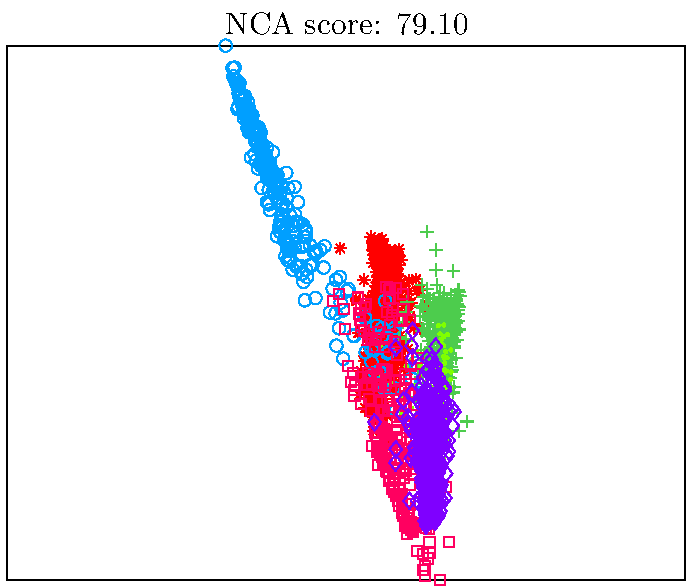
\includegraphics[width=0.45\textwidth]{images/nca-cs-nnzs-rand}}
			    \hspace{0.02\textwidth}
			 \subfigure[RCA initialization]{\label{fig:nca-sl-cs-rca}
\includegraphics[width=0.45\textwidth]{images/nca-cs-nnzs-rca}}
		\caption[Two dimensional projections of the \texttt{landsat} data set using the stochastic learning for the compact support NCA]{Illustration of final two-dimensional projections for the compact support NCA using stochastic learning. There were used two different initialization: random selection of parameters and RCA initialization.}
		\label{fig:landsat-projection}
	\end{figure}

\begin{table}
            	\centering
            	\begin{tabular}{lccc}
            	\toprule
            	Data set & Train & $1$-NN & NCA \\
            	\cmidrule(r){2-2}\cmidrule(r){3-4}
\texttt{usps}&$85.16 \pm 0.33$&$87.02 \pm 0.44$&$89.85 \pm 0.30$\\ 
\texttt{magic}&$76.92 \pm 0.56$&$79.09 \pm 0.42$&$82.92 \pm 0.36$\\ 
\texttt{mnist}&$80.55 \pm 0.28$&$81.96 \pm 0.26$&$86.36 \pm 0.18$\\ 
  \bottomrule
  \end{tabular}
  \caption[Accuracy scores for compact support NCA trained using stochastic learning on large data sets]{Accuracy scores for the compact support NCA method trained using stochastic learning on large data sets.}
  \label{tab:nca-cs-scores}
\end{table}

The compact support version of NCA is easy to implement and it is very fast as we already saw in section \ref{subsec:eval-comparison}. Usually only a small fraction of the points is inspected. In figure \ref{fig:nca-cs-nnzs}, we see how this fraction evolves with the learning process. In the first iterations there might be a larger number of points, but soon this drops off and stabilizes. It might be tempting to start with all the points very close together to ensure that no point is outside the compact support of any other point. This approach has however two drawbacks. Since all the points are in the support of all the other points it means the first iteration will not present any gain in speed. In fact, the first iteration can easily be as expensive as the whole learning process. A second issue is that the gradients will be very large and might ``throw away'' points out of the existing support. An initialization with RCA provided a more stable evolution. We also see that the final projection looks better in the second case (figure \ref{fig:landsat-projection}).

Results that demonstrate performance in terms of accuracy on small data sets are attached in appendix, tables \ref{app:tab:nca-cs-scores-1} and \ref{app:tab:nca-cs-scores-2}. The comparison has as baselines the classical NCA and the extended version of NCA with compact support kernels and background distribution (NCA CS BACK). The results on the large data set are available in table \ref{tab:nca-cs-scores}. 

\section{Recommendations}
\label{sec:eval-recommendations}

When dealing with a large data set, we suggest first trying the stochastic learning for the compact support NCA (NCA CS SL). This method has the advantage of being easy to implement and very fast even for large data sets. However, the speed does come at a cost. We note a slight decrease in accuracy for most experimentations. Nonetheless, applying the NCA CS SL first gives us an idea of how well NCA can perform on a given data set. If one is pleased with the score, it can use the NCA optimized using stochastic learning (NCA SL) or the more sophisticated approximate version that uses $k$-d trees. Usually, these last to methods get an improvement of a couple of percentages in accuracy over NCA CS SL\@. However all the methods offer better scores than the eigendecomposition.
